% ---
% Capa
% ---
\imprimircapa
% ---

% ---
% Folha de rosto
% (o * indica que haverá a ficha bibliográfica)
% ---
\imprimirfolhaderosto*
% ---

% ---
% Inserir a ficha bibliografica
% ---
% http://ficha.bu.ufsc.br/
%\begin{fichacatalografica}
%	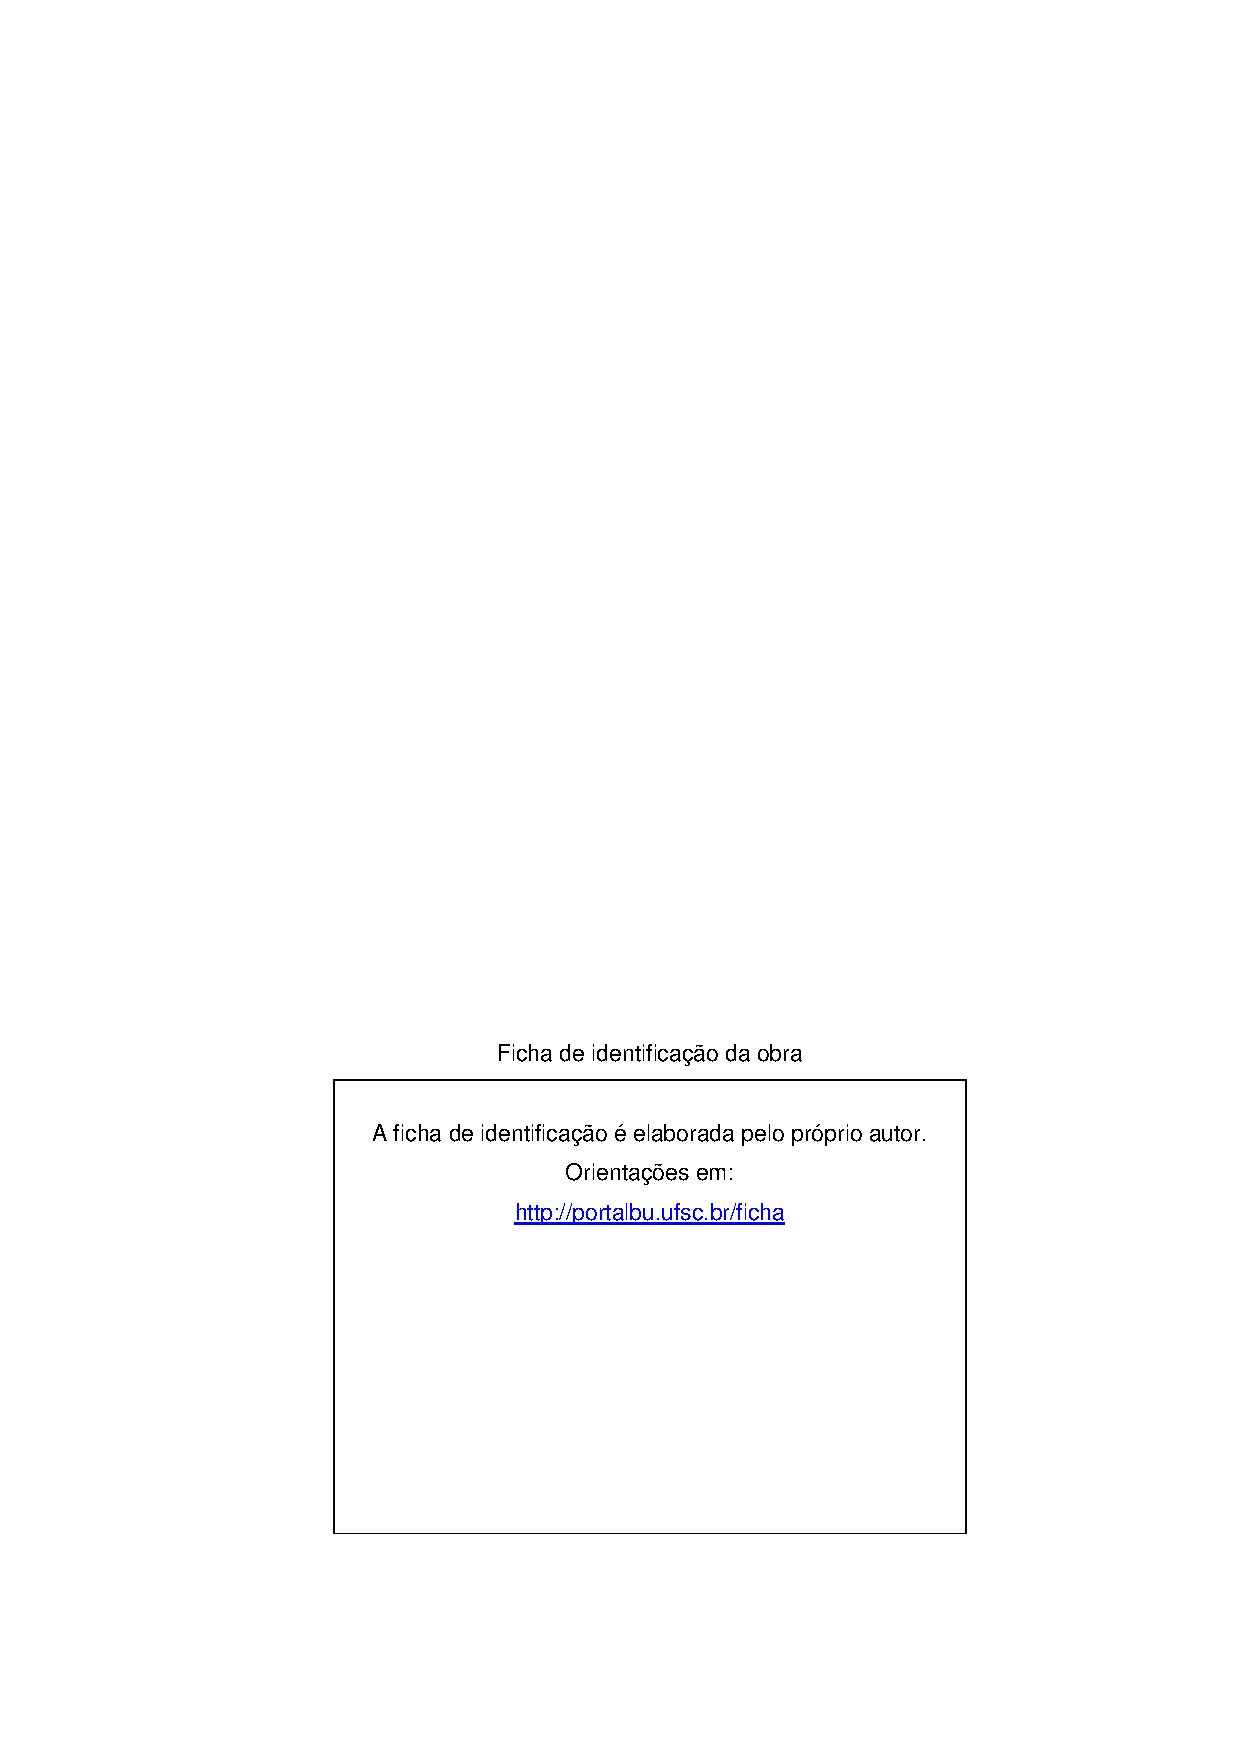
\includepdf{beforetext/Ficha_Catalografica.pdf}
%\end{fichacatalografica}
% ---

% ---
% Inserir folha de aprovação
% ---
%\begin{folhadeaprovacao}
	%\OnehalfSpacing
	%\centering
	%\imprimirautor\\%
	%\vspace*{10pt}		
	%\textbf{\imprimirtitulo}%
	%\ifnotempty{\imprimirsubtitulo}{:~\imprimirsubtitulo}\\%
	%		\vspace*{31.5pt}%3\baselineskip
	%\vspace*{\baselineskip}
	%\begin{minipage}{\textwidth}
	%% ~do~\imprimirprograma~do~\imprimircentro~da~\imprimirinstituicao~para~a~obtenção~do~título~de~\imprimirformacao.
	%Este~\imprimirtipotrabalho~foi julgado adequado para obtenção do Título de “\imprimirformacao” e aprovado em sua forma final pelo~\imprimirprograma. \\
	%	\vspace*{\baselineskip}
	%\imprimirlocal, \imprimirdata. \\
	%\vspace*{2\baselineskip}
	%\assinatura{\OnehalfSpacing\imprimircoordenador \\ %\imprimircoordenadorRotulo~do Curso}
	%\vspace*{2\baselineskip}
	%\textbf{Banca Examinadora:} \\
	%\vspace*{\baselineskip}
	%\assinatura{\OnehalfSpacing\imprimirorientador \\ %\imprimirorientadorRotulo}
%	%\end{minipage}%
%	\vspace*{\baselineskip}
%	\assinatura{Prof.(a) xxxx, Dr(a).\\
%	Avaliador(a) \\
%	Instituição xxxx}

%	\vspace*{\baselineskip}
%	\assinatura{Prof.(a) xxxx, Dr(a).\\
%	Avaliador(a) \\
%	Instituição xxxx}


%\end{folhadeaprovacao}

\begin{folhadeaprovacao}
	\OnehalfSpacing
	\centering
	\imprimirautor\\%
	\vspace{24pt}		
	\textbf{\imprimirtitulo}%
	\ifnotempty{\imprimirsubtitulo}{:~\imprimirsubtitulo}\\%
	%		\vspace*{31.5pt}%3\baselineskip
	\vspace*{\baselineskip}
	%\begin{minipage}{\textwidth}
	Este Trabalho de Conclusão de Curso foi julgado adequado para obtenção do Título de ``\imprimirformacao'' e aprovado em sua forma final pelo Curso de Graduação em Ciências da Computação.\\
	\vspace{12pt}
	\imprimirlocal, 11~de~dezembro~de~\imprimirano.\\
	
	\vspace*{18pt}
	\textbf{Banca Examinadora:}\\
	
	\vspace*{24pt}
	\assinatura{\OnehalfSpacing \imprimirbancaa}
	\vspace{6pt}
	Universidade Federal de Santa Catarina\\
	
	\vspace*{24pt}
	\assinatura{\OnehalfSpacing \imprimirbancab}
	\vspace{6pt}
	Universidade Federal de Santa Catarina\\
	
	\vspace*{24pt}
	\assinatura{\OnehalfSpacing \imprimirbancac}
	\vspace{6pt}
	Universidade Federal de Santa Catarina\\

    \vspace*{24pt}
	\assinatura{\OnehalfSpacing \imprimirbancad}
	\vspace{6pt}
	Universidade Federal de Santa Catarina\\
	
\end{folhadeaprovacao}

% ---

% ---
% Dedicatória
% ---
%\begin{dedicatoria}
%	\vspace*{\fill}
%	\noindent
%	\begin{adjustwidth*}{}{5.5cm}     
%		Este trabalho é dedicado aos meus colegas de classe e aos meus queridos pais.
%	\end{adjustwidth*}
%\end{dedicatoria}
% ---

% ---
% Agradecimentos
% ---
%\begin{agradecimentos}
%	Inserir os agradecimentos aos colaboradores à execução do trabalho. 
	
%	Xxxxxxxxxxxxxxxxxxxxxxxxxxxxxxxxxxxxxxxxxxxxxxxxxxxxxxxxxxxxxxxx. 
%\end{agradecimentos}
% ---

% ---
% Epígrafe
% ---
%\begin{epigrafe}
%	\vspace*{\fill}
%	\begin{flushright}
%		\textit{``Texto da Epígrafe.\\
%			Citação relativa ao tema do trabalho.\\
%			É opcional. A epígrafe pode também aparecer\\
%			na abertura de cada seção ou capítulo.\\
%			Deve ser elaborada de acordo com a NBR 10520.''\\
%			(Autor da epígrafe, ano)}
%	\end{flushright}
%\end{epigrafe}
% ---

% ---
% RESUMOS
% ---
% resumo em português
\setlength{\absparsep}{18pt} % ajusta o espaçamento dos parágrafos do resumo
\begin{resumo}
	\SingleSpacing
	
	%No resumo são ressaltados o objetivo da pesquisa, o método utilizado, as discussões e os resultados com destaque apenas para os pontos principais. O resumo deve ser significativo, composto de uma sequência de frases concisas, afirmativas, e não de uma enumeração de tópicos. Não deve conter citações. Deve usar o verbo na voz ativa e na terceira pessoa do singular. O texto do resumo deve ser digitado, em um único bloco, sem espaço de parágrafo. O espaçamento entre linhas é simples e o tamanho da fonte é 12. Abaixo do resumo, informar as palavras-chave (palavras ou expressões significativas retiradas do texto) ou, termos retirados de thesaurus da área. Deve conter de 150 a 500 palavras. O resumo é elaborado de acordo com a NBR 6028.

    % Nos últimos anos, tem-se testemunhado uma tendência de aumento no número de instituições de ensino superior, no ingresso de estudantes em cursos superiores e na quantidade de formandos no Brasil. Esse crescimento trouxe consigo desafios relacionados à validação da autenticidade de certificados acadêmicos — atualmente verificados de maneira predominantemente manual, um processo demorado, sujeito a erros e a aceitação de documentos fraudados.
    % Nesse contexto surge a Jornada do Estudante, um sistema disponibilizado pelo Ministério da Educação (MEC), que oferece, entre outras funcionalidades, o acompanhamento de registros acadêmicos de estudantes por meio de uma rede distribuída, de forma a garantir que apenas instituições de ensino digitalmente certificadas possam registrar créditos e certificações.
    % O presente trabalho de conclusão de curso revisita estratégias do estado-da-arte a respeito do uso de aprendizado de máquina na detecção de documentos falsificados, propondo um protótipo de solução que tem como base uma abordagem de aprendizado de máquina híbrida, por meio da \textit{clusterização}, detecção de anomalias e classificação de documentos de acordo com seu nível de inautenticidade.
    % Dessa forma, a integração dessa tecnologia à Jornada do Estudante possibilita a validação de documentos antes de seu registro na \textit{blockchain}, potencialmente garantindo maior segurança e confiabilidade no seu processo de inscrição.

    Nos últimos anos, no Brasil, o expressivo aumento do número de ingressantes, formandos e de instituições de ensino superior, trouxe consigo desafios relacionados à validação da autenticidade de certificados acadêmicos — atualmente verificados de forma predominantemente manual, sujeita a erros e falhas, como a aceitação de documentos fraudulentos.
    Nesse contexto, surge a Jornada do Estudante, um sistema disponibilizado pelo Ministério da Educação (MEC), que oferece, entre outras funcionalidades, o acompanhamento de registros acadêmicos de estudantes por meio de uma rede distribuída, de forma a garantir que somente instituições de ensino digitalmente certificadas possam registrar créditos e certificações.
    O presente trabalho de conclusão de curso revisita o estado-da-arte em detecção via aprendizado de máquina de documentos falsificados, além de propor um protótipo de solução híbrida, que combina análise multimodal, \textit{clustering}, detecção de anomalias e classificação de documentos de acordo com seu grau de legitimidade.
    Ao integrar esse sistema à Jornada do Estudante, é possível validar automaticamente os documentos antes de seu registro em \textit{blockchain}, aumentando significativamente a segurança e a confiabilidade do processo de credenciamento.

  

    \textbf{Palavras-chave:} segurança da informação, detecção de fraude, \textit{machine learning}, \textit{clustering}, detecção de anomalias, extração multimodal
\end{resumo}

% resumo em inglês
\begin{resumo}[Abstract]
	\SingleSpacing
	\begin{otherlanguage*}{english}

        In recent years, the significant increase in the number of higher education institutions, incoming students, and graduates in Brazil has brought challenges related to the validation of academic certificates’ authenticity—currently performed predominantly manually and prone to errors and failures, such as the acceptance of fraudulent documents. In this context, the Jornada do Estudante, a system provided by the Ministry of Education (MEC), was introduced; among other features, it enables the tracking of students’ academic records through a distributed network, ensuring that only digitally certified institutions can register credits and certifications. This undergraduate thesis revisits the state of the art in machine learning–based forgery detection for academic documents and proposes a hybrid prototype solution that combines multimodal analysis, clustering, anomaly detection, and document classification according to their degree of legitimacy. By integrating this system with the Jornada do Estudante, documents can be automatically validated before being recorded on blockchain, significantly enhancing the security and reliability of the credentialing process.
		
		\textbf{Keywords}: information security, fraud detection, machine learning, clustering, anomaly detection, multimodal feature extraction
	\end{otherlanguage*}
\end{resumo}




%% resumo em francês 
%\begin{resumo}[Résumé]
% \begin{otherlanguage*}{french}
%    Il s'agit d'un résumé en français.
% 
%   \textbf{Mots-clés}: latex. abntex. publication de textes.
% \end{otherlanguage*}
%\end{resumo}
%
%% resumo em espanhol
%\begin{resumo}[Resumen]
% \begin{otherlanguage*}{spanish}
%   Este es el resumen en español.
%  
%   \textbf{Palabras clave}: latex. abntex. publicación de textos.
% \end{otherlanguage*}
%\end{resumo}
%% ---

{%hidelinks
	\hypersetup{hidelinks}
	% ---
	% inserir lista de ilustrações
	% ---
	\pdfbookmark[0]{\listfigurename}{lof}
	\listoffigures*
	\cleardoublepage
	% ---
	
	% ---
	% inserir lista de quadros
	% ---
	%\pdfbookmark[0]{\listofquadrosname}{loq}
	%\listofquadros*
	%\cleardoublepage
	% ---
	
	% ---
	% inserir lista de tabelas
	% ---
	\pdfbookmark[0]{\listtablename}{lot}
	\listoftables*
	\cleardoublepage
	% ---
	
	% ---
	% inserir lista de abreviaturas e siglas (devem ser declarados no preambulo)
	% ---
	% \imprimirlistadesiglas
	% ---
	
	% ---
	% inserir lista de símbolos (devem ser declarados no preambulo)
	% ---
	%\imprimirlistadesimbolos
	% ---
	
	% ---
	% inserir o sumario
	% ---
	\pdfbookmark[0]{\contentsname}{toc}
	\tableofcontents*
	\cleardoublepage
	
}%hidelinks
% ---